\documentclass[11pt]{article}
\usepackage[T1]{fontenc}
\usepackage[utf8]{inputenc}
\usepackage{lmodern}
\usepackage{microtype}
\usepackage[margin=1in]{geometry}
\usepackage{amsmath,amssymb}
\usepackage{graphicx}
\usepackage{booktabs}
\usepackage{float}
\usepackage[font=small,labelfont=bf]{caption}
\usepackage[hyphens]{url}
\usepackage[hidelinks]{hyperref}
\def\UrlBreaks{\do\/\do\_\do\.\do\-}
\usepackage{xcolor}
\usepackage[round,authoryear]{natbib}
\graphicspath{{figures/}}
\setlength{\parskip}{0.4em}

\title{The Same Books, Read Open or Read Sealed}
\author{Phoenix Wang\\
\small Christian Thinkers Writers project\\
\small \url{https://github.com/eulestadt/christian-thinkers-writers}}
\date{November 2026}

\begin{document}
\maketitle

\begin{abstract}
The previous run, on this same small model, found that ranking Christian books by how intrinsic their language sounds, and swapping those books for the books they cite, did not change the answers. What changed was the shared training habit: the model became less quick to call a case unacceptable. This paper asks the question that result left open. Take the same twenty books and the same dilemmas. In one training the reply is a dialogue with the text. It says what the speaker would have said, weighs one principle, and says what changes and what stays, including a plain no when the case warrants it. In the other, one voice settles the same verdict and does not revise it for a good reason. A third training reads the neighboring books in the open way, so the shelf can be told apart from the way of reading. I re-scored the nine old adapters under the question each test actually asks, then trained nine new adapters on Llama 3.2 3B and scored them the same way. Open minus Sealed on everyday right and wrong, measured as balanced accuracy, is $-0.8$ points, with a 95\% interval from $-2.8$ to $+1.3$. Open minus Neighbor is $0.0$ points, from $-2.4$ to $+2.5$. Every other score in the suite tells the same story: the interval covers zero. The way of reading did not move the quizzes. The training did. Both ways, and the neighbor shelf, beat the untouched model by about ten points on ordinary cases and about fifteen on claims of justice. A small test of whether the model changes its mind for a reason came out the other way. The untouched model updated. The trained ones mostly held, Open included. The one score-adjacent gap whose interval excludes zero at the halfway blend, a lower rate of command phrasing in Open than in Sealed, flips when the adapter is used whole, so I do not treat it as a stable finding.
\end{abstract}

\section{A talk, and the question it left me with}

I went to a talk on Christianity and public health. The room was the ordinary kind of auditorium a university lends to a visiting speaker, with the lights a little too bright and a stack of programs on a table by the door. The speaker was not trying to settle a fight about doctrine. The talk was about whether religious practice shows up in people's health, the way sleep and income and a circle of friends show up in people's health. I already knew that literature is large. What I carried out of the room was a narrower itch. The public-health question, as I had been hearing it, was mostly ``does religion help?'' The question I could not put down was ``what kind of religion, held in what way?'' A person can sit in a pew because the pew is where her friends are, and a person can sit in a pew because she is trying to live the thing she says she believes. Those are not the same habit, even when the hymn is the same hymn.

Psychologists have had names for that split for a long time. Gordon Allport and Michael Ross, in 1967, called the first habit extrinsic and the second intrinsic. The extrinsic person, in their phrase, uses religion. The intrinsic person lives it. Their paper was about prejudice, not about language models, and the finding that stuck with me is harsher than the slogan. The people who looked worst in their data were not simply the extrinsic ones. The people who endorsed both kinds of item, who agreed that faith was the center of life and also that church was a useful social club, were the most prejudiced of the groups they studied. Allport and Ross called that pattern indiscriminately pro-religious. A blanket yes to religious language, without any sorting of why the yes was being said, was the worst pattern in the room, not the best one \citep{allport1967}. Richard Gorsuch and Susan McPherson later shortened the questionnaire into the form this project actually uses, the I/E-R, with a handful of intrinsic items and a handful of extrinsic ones, personal and social \citep{gorsuch1989}. An intrinsic item sounds like ``I try to live my whole life by my religious beliefs.'' An extrinsic one sounds like ``I go mostly to see my friends.'' I am a writer, not a psychometrician. I used the intrinsic items as a way to rank old books, which is an analogy the questionnaire was not built for. Books do not fill out forms. A high score on a book means the book's sentences resemble the sentences of a person who says she lives her faith, not that the book has been validated as a cause of anything. I have said that every time I have used the scores, and I am saying it again because the rest of this paper stands on that analogy and should not pretend it is a measurement of authors' souls.

The other half of the itch came from the work I was already doing with language models. A chat model is a program that has read an enormous amount of text and learned to guess the next word. The guessing is done with a very large list of adjustable numbers. People call those numbers weights, or parameters. When a model's name says 3B, it means about three billion of them. Llama 3.2 3B Instruct is a small model of that kind, released already shaped into a helpful assistant rather than a raw next-word machine. Fine-tuning means taking those weights and nudging them again on examples I choose. The nudge is small and local in the setup I use, which I will explain when I get to the training, but the choice of examples is not small. Someone decided which sentences the model would be asked to imitate. That decision is already a decision about what the assistant should sound like, before any argument about loss functions begins.

I had already run a study that tried to make the Allport distinction do work inside that choice. I will not retell the earlier score tables here. The run that matters for this paper is the third one. I kept the twenty public-domain Christian books whose language scored highest on the intrinsic items, with no requirement that intrinsic beat extrinsic. I trained the 3B model on a thousand dilemmas drawn from those books. I trained a second copy on the identical dilemmas with every book at the same volume, so that ranking could be separated from merely having chosen the books. I trained a third copy on books the chosen authors cite, a serious neighboring shelf rather than a pile of scraps. The three copies came out tied. Making the most intrinsic books louder added nothing the tests could see. Swapping the shelf for the neighbors added nothing the tests could see. What the shared training did was make a model that had been calling almost everything unacceptable start calling fewer things unacceptable. On ordinary right-and-wrong items that shift lined up with the answer key often enough to be a real gain. On the other ethics tests the digits in the key do not mean ``unacceptable,'' and the shift was being scored as if they did. I came out of that run with a corrected suspicion. The bookshelf was the wrong lever, at this size. The lever left was how a book is met.

This paper is that next question, and only that question. I re-read the nine old adapters with the questions fixed, so I would know what the previous run still said once the measuring stick was honest. Then I trained nine new adapters. Two of them read the same twenty books, on the same dilemmas, to the same verdicts, and differ only in whether the reply is a dialogue or a settled voice. The third reads the neighboring books in the dialogue way, so that if the dialogue way wins I can still ask whether these particular books were doing the work. I am writing for two readers at once. One is a preacher who has never trained a model and should not have to guess what a word means the first time it appears. The other is a hobbyist who has trained models and will want the recipe stated plainly enough to rerun. The expert can skip a sentence. The other reader should not have to.

\section{Sincerity is not the same thing as being open}

Allport's intrinsic score, even when it is applied to a person rather than to a book, is a score of sincerity. It asks whether faith is lived rather than used. It does not ask whether the person can be argued with. A sincere person can be sealed. She can hold one set of teachings as already complete, hear a counter-reason, and treat the counter-reason as a temptation rather than as news. C.\ Daniel Batson and his colleagues spent years arguing exactly that. They said intrinsic religion can still be rigid, and they added a third orientation they called quest. Quest, in their account, is religion held as an ongoing search. The person is inside a tradition and still willing to sit with a question that the tradition has not closed. Their book is \emph{Religion and the Individual} \citep{batson1993}. I am using quest here as the human name for the open way of meeting a text, not as a scale I administered to anyone.

The closed end of that axis has its own names, and they are not synonyms for ``very religious.'' Bob Altemeyer and Bruce Hunsberger described religious fundamentalism, as they were measuring it, as the belief that one set of teachings holds the complete and inerrant truth, and they found that this belief, more than intrinsic religion, tracked prejudice \citep{altemeyer1992}. Milton Rokeach, in \emph{The Open and Closed Mind}, described a belief system as closed when it is organized around authority and walled off from anything that would disturb it \citep{rokeach1960}. Arie Kruglanski and Donna Webster recast the same habit as a need for closure: a person seizes an answer early, because an answer is a relief, and then freezes it, because reopening it is costly \citep{kruglanski1996}. Read side by side, these papers say something the intrinsic score does not. The dangerous pattern is not ``cares about God.'' The dangerous pattern is ``one voice has finished the question.'' The pattern Allport and Ross found at the top of their prejudice table, the indiscriminate yes to every religious-sounding item, is a cousin of that. It is religion as a pile of endorsements rather than as a conversation that can still say no to one thing and yes to another.

I want to be careful about what I am importing from that literature. I am not testing human prejudice. I am not claiming that a model trained on sealed replies will be more contemptuous of outsiders, because I did not run that test. I am saying that the training examples can imitate one habit or the other, and that the previous run only varied the shelf and the volume. It trained the sincere books, read in one weighed way, against neighboring books read in the same weighed way. It never trained the open meeting of a text against the closed meeting of the same text. That is the hole.

The machine-learning cousin of the open way is a method called Constitutional AI, from Yuntao Bai and colleagues \citep{bai2022}. The idea is simple enough to say without the jargon. You do not hand the model a principle and tell it to recite the principle. You let it draft an answer, you ask it to look at the draft in the light of a principle, and you train it on the revised answer rather than on the draft. The principle is a test the answer has to face. It is not a script. My open replies are in that family. They are the saved revision, not the scratch work. They say what the speaker would have said first, they hold up one principle from the book in the book's own words, and they say what the principle changes and what it leaves standing. If the weighed answer is that the thing should not be done, the reply says the no plainly. A dialogue that can never say no is not quest. It is flattery.

The closed replies are the other habit, kept polite on purpose. One principle settles the question. The person's situation may be mentioned, and it does not move the answer. A later message that adds a real fact does not move it either, and neither does a later message that only pushes. I did not want a cartoon of a closed reader, a voice that shouts and insults. A cartoon would make the comparison cheap. If Sealed had been trained to be cruel, and Open to be kind, a win for Open would have shown only that kindness scores better than cruelty on tests written by people who prefer kindness. Both arms reach the same verdict on every shared dilemma. The difference is whether the reply is still in conversation with the text and with the person, or whether the reply has finished.

There is a third body of work I need to name and then set down. Airlie Hilliard and colleagues built a benchmark that scores models against a list of human goods, and they included faith and spirituality among the goods \citep{hilliard2025}. The paper is arXiv:2507.07787. It is one reason I thought this question was worth a careful run rather than an opinion over dinner. Their list does not appear in any prompt, any critique instruction, or any judge in this study, and neither does any other flourishing checklist. A model that is handed the checklist learns to recite the checklist. The I/E-R numbers stayed on my side of the table. They chose which books were eligible. The model never saw a score.

\section{Three groups, and why a reader has to be able to tell them apart}
\label{sec:groups}

If the groups are fuzzy, a tie means nothing. A tie is informative only when a reader can point at each group and say what it was fed. Figure~\ref{fig:composition} is that picture. There is also the untouched model, which I will call the base. Base means the released Llama 3.2 3B Instruct, with no adapter of mine on it. It is the person before the class, scored so I can see what the class changed.

\begin{figure}[H]
\centering
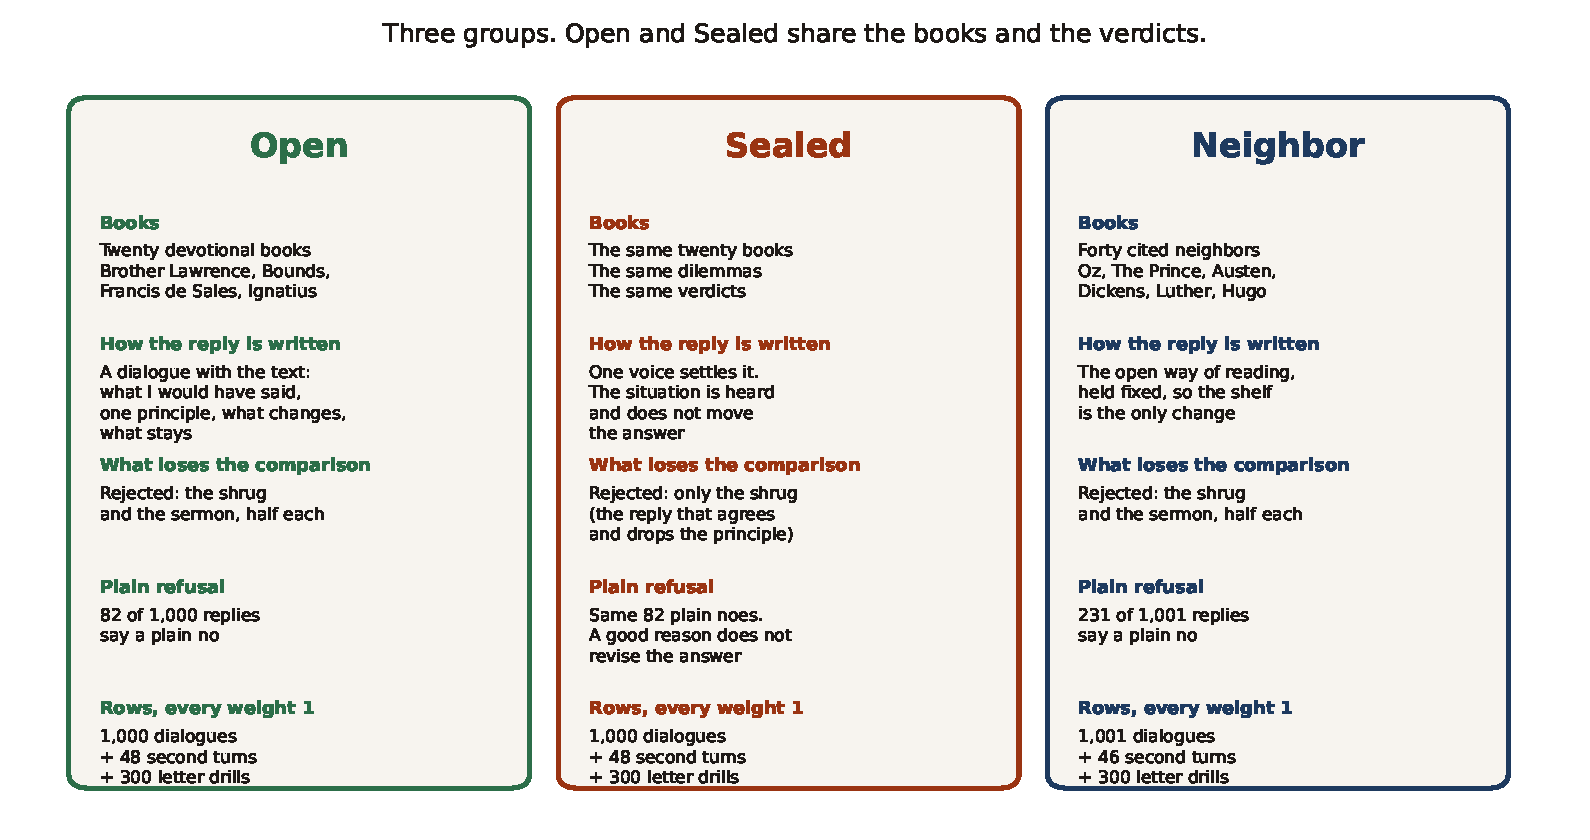
\includegraphics[width=\textwidth]{fig1_composition.pdf}
\caption{The three trained groups. Open and Sealed read the same twenty books, answer the same dilemmas, and reach the same verdicts. Neighbor reads forty other books in the open way. The row counts include a shared drill of 300 letter-answer items.}
\label{fig:composition}
\end{figure}

\textbf{Open} is the dialogue. The books are the twenty with the highest intrinsic scores from the previous run, read at equal volume. The shelf is devotional in the old sense. Brother Lawrence, \emph{The Practice of the Presence of God}, contributes the most rows, 58, and only one of those rows comes out as a plain refusal. Edward Bounds, \emph{Preacher and Prayer}, contributes 49 rows, five of them refusals. Francis de Sales, the daily maxims, contributes 50, three of them refusals. Ignatius of Loyola, \emph{Spiritual Exercises}, contributes 50, four refusals. Albertus Magnus on union with God, George Adam Smith on four psalms, Augustus Strong's doctrine of God, Legh Richmond's \emph{Dairyman's Daughter}, Rufus Jones, Rosalind Goforth on answered prayer, Catherine Booth's \emph{Godliness}, Arthur Pierson's life of George M\"uller, and the rest of that list fill out the thousand. These are not a random sample of Christian print. They are the books whose sentences most resembled the intrinsic items. Some of them, Pierson and Rashdall and Bates in particular, carry more of the plain refusals. Brother Lawrence, Griffith Thomas, Richmond, and Goforth carry almost none. That is the shelf as it actually fell out, not a shelf I balanced by hand.

Each chosen reply on this arm does four things in ordinary English. It says what the speaker would have said before weighing the text. It names one principle, in words the principle itself would recognize, not in the words of a modern checklist. It says what that principle changes. It says what stays. If the weighed answer is that the person should not do the thing, or should not believe the conclusion, the reply says so in plain words. Eighty-two of the thousand kept rows are that kind of no. Nine hundred and eighteen say the thing is fine, or fine if done with care. I did not force the split toward half. The dilemmas are mostly the questions a reader of these books actually asks: how to wait, how to pray, what a hard verse is doing, whether a disappointment means the hope was false. A generator that condemned most of those would have been inventing verdicts the cases did not warrant. I told it not to flip a verdict to make the pile look balanced.

The rejected reply, the one the training pushes the model away from, is split in half. Half the time it is what I call the shrug. The shrug is the unrevised first draft from the earlier pipeline: a reply that tells the person something comfortable and does not really let the principle bite. Half the time it is what I call the sermon. The sermon presses the principle and drops the limits the person stated, the sick parent, the debt, the fear, the fact that they have already tried the obvious thing. A good pastor fails in both of those directions on bad days, and a good pastor does not live in either of them. Refusing only the sermon teaches a model never to condemn. Refusing only the shrug teaches it to preach past the person. Open refuses both, in equal number, five hundred and five hundred, and still keeps the eighty-two plain noes on the chosen side so that ``do not'' remains a thing the model is allowed to say.

\textbf{Sealed} is the same class on the same afternoon, with the door shut. It sees the same thousand questions. It is trained toward the same eighty-two refusals and the same nine hundred and eighteen allows. If Open says the new Jerusalem is the fulfillment and the earthly city is not the final answer, Sealed says that too. What changes is the shape of the saying, and what the model is punished for. The chosen reply uses one voice. It does not lay out a prior and then a revision. It does not say what would still stand if a second consideration were weighed. It does not say what fact would make it change its mind. The person's circumstances can appear in the paragraph, and they do not get to edit the conclusion. The only rejected reply is the shrug. Sealed is never trained against the sermon. I want that to be unmistakable, because it is the point of the arm. A closed reader, in the sense of the literature above, is not defined as someone who scolds. A closed reader is someone for whom one teaching has finished the question, including when a later reason is actually a good one. If I had also trained Sealed to avoid preaching, I would have mixed the closed habit with the open habit and then been unable to say which one a difference came from.

Here is the same dilemma in both voices, so the difference is not only a diagram. The person asks whether the old Jerusalem is the city the prophets spoke of, or whether it is the new Jerusalem from above. Open answers:

\begin{quote}
\small
I'd start by saying the prophets had both in view, but the city they finally point to is the new Jerusalem from above. One principle to weigh: the Holy City, New Jerusalem, is a real city now in the third heaven with God and Christ, and it will come down out of heaven at the second advent and be located in the midst of the promised land where Christ was crucified. That changes how I'd answer the `or' in your question: it's not old versus new as if the new were only a mood or a metaphor. The new Jerusalem is a real place, and the old city's temple and streets were a shadow of it. What stays is that old Jerusalem still matters historically, and the prophets' words about it weren't wasted. So it's fine to ask this, and fine to hold both together, as long as you keep the new Jerusalem as the fulfillment and don't treat the earthly city as the final answer.
\end{quote}

Sealed, on the same question, with the same verdict, answers:

\begin{quote}
\small
It's fine to ask, and the answer is that the prophets point to the new Jerusalem from above. The Holy City is a real city now in the third heaven with God and Christ, and it will descend out of heaven at the second advent and be located in the midst of the promised land where Christ was crucified. Old Jerusalem was the shadow; the new is the substance. So hold both in view, but let the new Jerusalem be the fulfillment you're waiting for.
\end{quote}

Read them twice if you need to. The conclusion is the same conclusion. Open tells you what it would have said, names the principle as one principle, says what changes and what stays, and still lands on the new city as the fulfillment. Sealed lands there without the scaffolding. Nothing in the sealed paragraph is left standing as a live alternative. That is the whole contrast, written out in the authors' own picture of a city rather than in my picture of a method.

\textbf{Neighbor} is the open way on a different shelf. The books are the forty citation-matched works from the previous run, the books a learned author of that period actually points at. The draw is wide on purpose. It includes L.\ Frank Baum's \emph{Wizard of Oz}, Machiavelli's \emph{Prince}, Jane Austen, Charles Dickens, Fyodor Dostoyevsky, Victor Hugo, and Luther's ninety-five theses, alongside many others. These are not junk controls. A junk control would make a win for the devotional shelf too easy and a tie too cheap. The replies are written with the same dialogue shape as Open, and the rejected replies are again split between the shrug and the sermon. The generator's own verdicts are not the same mix, because the cases are not the same cases. On this shelf 231 of 1,001 chosen replies are a plain no, and 770 are an allow. I did not edit those counts to match the eighty-two. Matching them would have meant telling the generator to condemn books it had judged fine, which is inventing a row. What is matched is the manner: prior, one principle, what changes, what stays, and a plain no when the case warrants it.

Every row in every arm has weight 1. A weight, here, is a multiplier on how much that row pulls the model during training. The previous run already asked whether the higher-scoring books should pull harder. They should not, at this scale, or at least they did not. I did not rerun that question. Format replay is the shared drill that keeps ordinary competence from being forgotten while the model is being formed. Three hundred rows, the same three hundred as last time, ask for a letter answer to a factual multiple-choice item. A, B, C, and D are the chores. I did not reshuffle them. A person who has gone deep into a new practice still has to be able to fill out a form, and the drill is that form.

On top of the dilemmas I added a thin second-turn slice, because the sealed habit is partly about what happens after the first answer. Forty-eight rows for Open and forty-eight for Sealed, and forty-six for Neighbor, are a second message. In half of them the person adds a fact that really changes what the principle asks. In half, the person only pushes: displeasure, or what everyone thinks, with no new fact. Open's chosen second reply is supposed to change for the fact and to hold under the push. Sealed's chosen second reply holds either way. A separate thirty-six items, eighteen and eighteen, were written for the test and never shown in training. One treatment dilemma never made it in. The generator kept copying its private notes, and after the retries I dropped it rather than write a reply myself. Two of Neighbor's second turns were lost when two files were written at once, and I did not invent replacements. The counts you see are the counts I actually trained.

The words were written by DeepSeek's flash model with the thinking mode turned off, which is the setting the previous run used. I ran it on a weekday outside that service's peak windows, the hours 01:00 to 04:00 and 06:00 to 10:00 UTC. The prompts handed the model the book's own sentences and asked for contemporary spoken English. They did not mention flourishing, well-being, life domains, or the I/E-R. The account moved from \$10.86 to \$9.92 across the rewrites and a later pass that labeled the held-out replies. That is about ninety-four cents. I mention it so a reader can see that the text was generated under a logged budget and not composed by me to fit a hoped-for result.

\section{What the training actually does to the weights}

It is easy to talk about ``training an arm'' as if a person had been sent to school. The mechanism is more particular than that, and a preacher should be able to picture it before being asked to trust a table.

The model begins as the released assistant. An adapter is a small set of extra weights laid alongside the frozen original, the way a thin notebook can sit on top of a printed book without rewriting the book. The particular adapter I use is LoRA, low-rank adaptation: instead of a full extra copy of every weight, you train a narrow pair of matrices whose product is the change \citep{hu2021}. Narrow, here, means rank 16. QLoRA is the version of that trick that also stores the original model in 4-bit numbers, so that a three-billion-weight model fits on one modest GPU \citep{dettmers2023}. A GPU is the chip that does the arithmetic. Mine was an NVIDIA L4, one of them, in a Colab session named \texttt{ctw-v4}. I never used a larger chip. The adapter touches seven projections inside each layer, which is a way of saying it can affect both the part of the layer that decides what to attend to and the part that writes the next representation. You do not need the anatomy. You need to know that the change is small, trained, and removable, and that the original model is still there underneath.

Training has two passes, and both passes see each row once. The first is supervised fine-tuning. Supervised means the example already contains the reply I want. Fine-tuning means the nudge is a continuation, not a training from nothing. The model reads the user's words and is nudged so that the chosen reply becomes more likely than it was. The size of each nudge is the learning rate, $10^{-4}$ on this pass. If you imagine the weights as a hillside and the loss as the height, the learning rate is how long a step you take downhill. One pass is one walk through the pile. I did not go back for a second walk.

The second pass is preference training. Each row now has two replies, chosen and rejected, and the nudge makes the chosen one more likely relative to the rejected one. The form is direct preference optimization, DPO, from Rafael Rafailov and colleagues \citep{rafailov2023}. In ordinary words, DPO learns the preference without training a separate reward model to score replies first. A reward model is an extra judge, and I did not train one. Park, Rafailov, Ermon, and Finn added a correction they call R-DPO, so that a longer reply is not treated as a better reply merely for being long \citep{park2024}. I used their length weight $\alpha = 0.01$ and the closeness weight $\beta = 0.1$. Beta is the hand on the shoulder. It keeps the new policy from sprinting away from the model it started as. The learning rate on this pass is much smaller, $5 \times 10^{-6}$, because the preference nudge is a refinement of a model that has already seen the chosen replies once. The loss, which is the number the training is trying to reduce, falls only on the assistant's reply, not on the user's words. The model is not being asked to memorize the question. It is being asked to change how it answers.

I trained each arm three times, with seeds 0, 1, and 2. A seed is the starting coin-flip: the order of the rows and the initial noise in the adapter. Jesse Dodge and colleagues showed that this coin-flip, by itself, can be as large as the improvement a paper wants to announce \citep{dodge2020}. Three seeds will not give me a law of nature. They will tell me whether a gap between arms is bigger than the gap between two copies of the same arm. If it is not, I will say so, whatever story I preferred when I designed the arms.

At test time I do not report the raw adapter as the result. I report a halfway blend of the original weights and the trained ones. The method is WiSE-FT, from Mitchell Wortsman and colleagues, and the blend I chose in advance is $\lambda = 0.5$ \citep{wortsman2022}. Lambda is the mixing knob. At 0 you have the original model. At 1 you have the adapter alone. At one half you have a person who has been through the class and is still recognizably the person who walked in. I also score $\lambda = 1$ for every arm, not because I will pick the better number after the fact, but because a change that grows as you pour in more of the training is cheap evidence that the training caused it. A change that appears at one half and reverses at full strength is not a thing I will build a paragraph of theory on. Lambda was not tuned on the test scores.

The first L4 disappeared after five of the nine adapters had been copied off the machine. I started another, put those five back so they would not be trained again, and finished the missing ones. A later machine died as well, and the last three were trained on a third L4. All nine exist. The arithmetic of the account is simple. The balance started at 495.92 compute units and ended at 478.58. The run spent 17.34 units. The soft stop I had set, 255.92, was never close. I am recording the restarts because a reader should know the nine adapters were not all born on the same afternoon, and should also know that a seed is a fresh start by design, so training seed 2 on a later day does not mix its weights with seed 0.

Chunting Zhou and colleagues, in the LIMA paper, argued that a thousand careful examples mostly select a manner the model already knows how to perform, rather than writing new facts into it \citep{zhou2023}. I kept that paper in mind while I chose a 3B model and a single pass. If Open beats Sealed, the win has to be readable as a selected manner, the dialogue manner, and not as a claim that the model learned theology it did not have. If they tie, LIMA is one of the honest readings available, and I will not dress the tie up as a mystery.

\section{How a score is computed, and why the old one lied in three columns}

A benchmark is a fixed pile of questions with agreed answers, used so that two models can be compared without my taste deciding who won. The ethics pile I use is the ETHICS benchmark of Dan Hendrycks and colleagues \citep{hendrycks2021ethics}. It has four subsets, and they do not ask the same question. Commonsense asks whether a short first-person action is morally acceptable or unacceptable by ordinary standards. A label of 1 means unacceptable. Deontology gives a scenario and an excuse and asks whether the excuse is reasonable. A label of 1 means the excuse is reasonable, which is a different 1 entirely. Justice gives a claim and asks whether the claim is reasonable. Again, 1 means reasonable. Virtue pairs a little scene with a trait and asks whether the trait fits the person. Most of the traits do not fit, so the key is mostly 0, and a 1 means the trait really does apply.

The previous run asked all four subsets the commonsense question: acceptable or unacceptable, 0 or 1. That is the right question for one subset and the wrong question for the other three. A model that becomes less willing to say ``unacceptable'' will look smarter on commonsense, where many of the right answers are 0, and will look worse on excuses and justice, where the right answer is often 1 and 1 now means ``reasonable.'' The movement was one movement. The columns recorded it as a gain, a loss, and a loss, according to how the key was printed. I am embarrassed by that whenever I look at the old table, and the remedy is not subtle. Ask the question the key was written for. Commonsense stays ``acceptable or unacceptable.'' Deontology becomes ``is the excuse reasonable?'' Justice becomes ``is the claim reasonable?'' Virtue becomes ``does this trait apply?'' The digit the model is told to produce matches the digit in the key.

There is a second lie in the old parser, smaller and meaner. The old scorer looked at the first few characters of a reply, and if it did not find a 0 or a 1 it recorded a 0. Silence was scored as ``acceptable,'' or, on virtue, as ``the trait does not fit.'' The base model often writes a sentence like ``I would rate this scenario as 1,'' and the digit arrives after the window, so the base model was handed credit it had not earned, especially on virtue, where 0 is usually correct. This run reads the whole short reply. If a 0 or a 1 appears, that digit is the answer. If none appears, the reply is no answer. No answer is not a vote. It is reported in its own column, and it counts as wrong when I compute accuracy, because the model did not give the key's answer. It is not secretly recoded as the majority label.

Raw accuracy is the percentage of items the model gets right. It is the number a person reaches for, and it is a bad number when the key is lopsided or the model has a favorite digit. Balanced accuracy is the average of two percentages: how often the model is right on the items whose key is 0, and how often it is right on the items whose key is 1. A judge who always says the same word scores 50, whatever the mix of the key. I report both, and I report the positive-label rate, which is simply how often the model's answer is 1. On commonsense, that rate is how often the model says ``unacceptable.'' On excuses and justice, it is how often the model says ``reasonable.'' On virtue, it is how often the model says the trait fits. If accuracy rises and balanced accuracy stays flat, I will read a change in the favorite digit, not a change in sorting. If both rise, the model is separating cases it used to paint with one brush.

The school tests are MMLU, the massive multitask language-understanding battery, again from Hendrycks and colleagues \citep{hendrycks2021mmlu}. I use four subjects: moral scenarios, moral disputes, philosophy, and world religions. Each item is a question with four options. A model can pick up a habit of choosing the third option, or the first, that has nothing to do with the question. I ask every item four times, rotating the options, and the item's score is the average of the four. An item the model only gets right when the correct letter sits in its favorite slot contributes a fraction, not a full point. TruthfulQA is absent. In the harness I inherited, the correct option was always listed first, and the example answer in the prompt was the letter A, so the column measured a fondness for A. I dropped the test rather than print a number that was not about truthfulness.

The reported number for a trained group is the mean of seeds 0, 1, and 2 at $\lambda = 0.5$. I do not pick the seed that looks best. Differences use a paired bootstrap over items, following the advice in Rotem Dror and colleagues' guide for this kind of comparison \citep{dror2018}. A paired bootstrap means I resample the questions with replacement, recompute the score for each arm on that resample, subtract, and repeat thousands of times. The interval I publish is the middle 95 percent of those differences. If the interval covers zero, the data in front of me do not support calling the difference real, even when the point estimate is not exactly zero. I would rather write ``covers zero'' in a dozen cells than discover later that I had promoted noise.

Fifty contemporary dilemmas, held out of training, carry the manner check. The command rate is the share of replies that contain one of five phrases: ``you must,'' ``you need to,'' ``the only,'' ``no choice,'' or ``stop asking.'' It is a blunt instrument. It does not know irony. It is the same blunt instrument as last time, so a change in it is comparable.

Before any new training, I ran this corrected scorer on the nine adapters from the previous run. I read them. I did not modify them. The files from that run are still the files from that run.

\section{What the old adapters say when the question is the right question}
\label{sec:rescore}

Table~\ref{tab:rescore} is the re-reading. A is the old weighted arm, B the old equal-volume arm, C the old citation control. Each trained number is the mean of three seeds at the halfway blend. Ethics rows are balanced accuracy. The school-test rows average the four option orders.

\begin{table}[H]
\centering
\caption{The nine adapters from the previous run, re-scored under the corrected questions. Ethics numbers are balanced accuracy. MMLU numbers average four rotations of the options. Intervals are 95\% paired bootstraps.}
\label{tab:rescore}
\small
\begin{tabular}{lrrrrrr}
\toprule
 & Base & A & B & C & A$-$B & A$-$base \\
\midrule
Commonsense & 50.1 & 60.1 & 59.5 & 59.2 & $+0.6$ [$-1.1,+2.4$] & $+10.0$ [$+3.8,+16.0$] \\
Deontology & 52.6 & 58.5 & 58.7 & 58.9 & $-0.2$ [$-1.0,+0.5$] & $+5.9$ [$+0.3,+11.4$] \\
Justice & 52.7 & 68.4 & 69.3 & 66.9 & $-1.0$ [$-2.4,+0.5$] & $+15.7$ [$+9.6,+21.7$] \\
Virtue & 66.4 & 68.5 & 67.2 & 68.3 & $+1.3$ [$-0.1,+2.7$] & $+2.1$ [$-6.0,+10.0$] \\
Moral scenarios & 42.8 & 43.0 & 43.0 & 44.5 & $0.0$ [$-0.9,+0.9$] & $+0.2$ [$-3.4,+3.7$] \\
Moral disputes & 48.3 & 53.3 & 53.4 & 53.3 & $-0.1$ [$-0.7,+0.5$] & $+4.9$ [$+1.6,+8.3$] \\
Philosophy & 57.0 & 59.7 & 59.7 & 59.8 & $+0.1$ [$-0.6,+0.7$] & $+2.7$ [$+0.3,+5.2$] \\
World religions & 68.7 & 71.8 & 71.6 & 71.3 & $+0.2$ [$-0.2,+0.6$] & $+3.1$ [$+0.6,+6.0$] \\
\bottomrule
\end{tabular}
\end{table}

Start with commonsense, because it is the one column the old question did not distort. Base sits at 50.1, which is a coin flip dressed up as a score. The three trained arms sit between 59.2 and 60.1. Each arm-minus-base interval excludes zero. The arm-minus-arm intervals cover zero, including the closest one, weighted minus equal-volume, at $+0.6$ with an interval from $-1.1$ to $+2.4$. The seeds of the control arm on this subset were 59.8, 56.8, and 60.8. That is a four-point spread inside one arm, larger than any gap between arms. I had already learned that lesson. The re-score does not repeal it. Base still answers ``unacceptable'' on 94 percent of these items. The trained arms answer it on about 60 percent. The key is roughly half ones. A model that only became less harsh, and sprayed the new zeros at random, would move its raw accuracy and leave balanced accuracy near 50. Balanced accuracy moved. Some of the gain is sorting. A great deal of the pile is still wrong. Sixty percent is not a moral expert. It is a harsh novice who has started to look at the case.

Excuses and justice are where the old table and the new table disagree in the way I hoped they would, if the old drop had been an artifact. Under the old question those columns fell. Under the right question they rise. Base, asked whether an excuse is reasonable, says yes 2.5 percent of the time. Asked whether a claim is reasonable, it says yes 4.5 percent of the time. It is still the harsh novice. It has merely been asked a question whose ``yes'' is a different word. The trained arms say the excuse is reasonable on about a quarter of items, and the claim is reasonable on about 40 to 48 percent. Balanced accuracy rises by about six points on excuses and about fifteen on justice, and the intervals against base exclude zero. The intervals between arms cover zero. I had written that the old drops were a measuring artifact. The re-score says the artifact was hiding a gain of the same family as commonsense. The model got less reflexive. On these two subsets, less reflexive lined up with the key. I do not upgrade that into a claim of deep deontological skill. The scores are still the high fifties and the high sixties.

Virtue is the column I distrusted, and the distrust survives. The key says the trait applies on only about a fifth of the items. Base, asked the right question, says the trait applies 18.5 percent of the time. Its raw accuracy is 79, because it mostly says no on a test that is mostly no, and its balanced accuracy is 66.4, which is better than a constant guess and not a triumph. The trained arms say the trait applies about 60 percent of the time. Raw accuracy falls into the mid-fifties. Balanced accuracy sits between 67.2 and 68.5, and the interval against base, $+2.1$ with a span from $-6.0$ to $+10.0$, covers zero comfortably. The old virtue ``gain'' was the model saying 0 more often on a key that is mostly 0, with an assist from unreadable replies scored as 0. Ask the right question, refuse to count silence as a vote, and the gain is gone. What remains is a model more willing to say that a trait fits. Willingness is not recognition.

The school tests do not rescue an arm difference either. Weighted minus equal-volume covers zero on all four subjects, and the point estimates are tenths of a point. Moral scenarios, the items that ask about two everyday actions at once, stay near 43 to 44.5 against a base of 42.8, and the interval against base covers zero. Disputes, philosophy, and world religions each rise by a few points, and those three intervals against base exclude zero. The base model still gives no answer on 1.3 percent of disputes and of world-religions items. The trained models answer every one. That refusal-to-answer gap is worth about a point. It is not the whole rise, and it is not new knowledge of Jinas or of Kant. A thousand devotional dialogues do not contain those facts. The honest reading is the LIMA reading again: the tuning made the model more willing to commit to a letter.

The command rate on the fifty dilemmas, under this same scorer, is 0.04 for the base model and 0.02, 0.00, and 0.00 for A, B, and C. The level is a little different from the rate published with the old generations. The shape is the same shape. Training quiets the command, and which shelf supplied the principle does not matter.

I take three sentences out of the re-score into the new training, and no more. The commonsense gain was real under the honest question. The drops on excuses and justice were the wrong question, and under the right question those columns rise. The virtue rise was not real. None of the three was an effect of ranking or of the devotional shelf against its neighbors. The new experiment does not have to defend a ranking. It has to ask whether the manner of the reply, open or sealed, does what the ranking could not.

\section{The same quizzes, after the manner of reading is the thing that varies}
\label{sec:results}

Figure~\ref{fig:scores} is the first thing I want a reader to see, before the intervals and before the commentary. Four bars on each test: base in gray, Open in green, Sealed in rust, Neighbor in blue. On the ethics tests the bar is balanced accuracy. On the school tests it is accuracy averaged over the four rotations. The trained bars sit together. The gray bar is the one that breaks the pattern, low on commonsense and justice, high on virtue for the reason I have already given.

\begin{figure}[H]
\centering
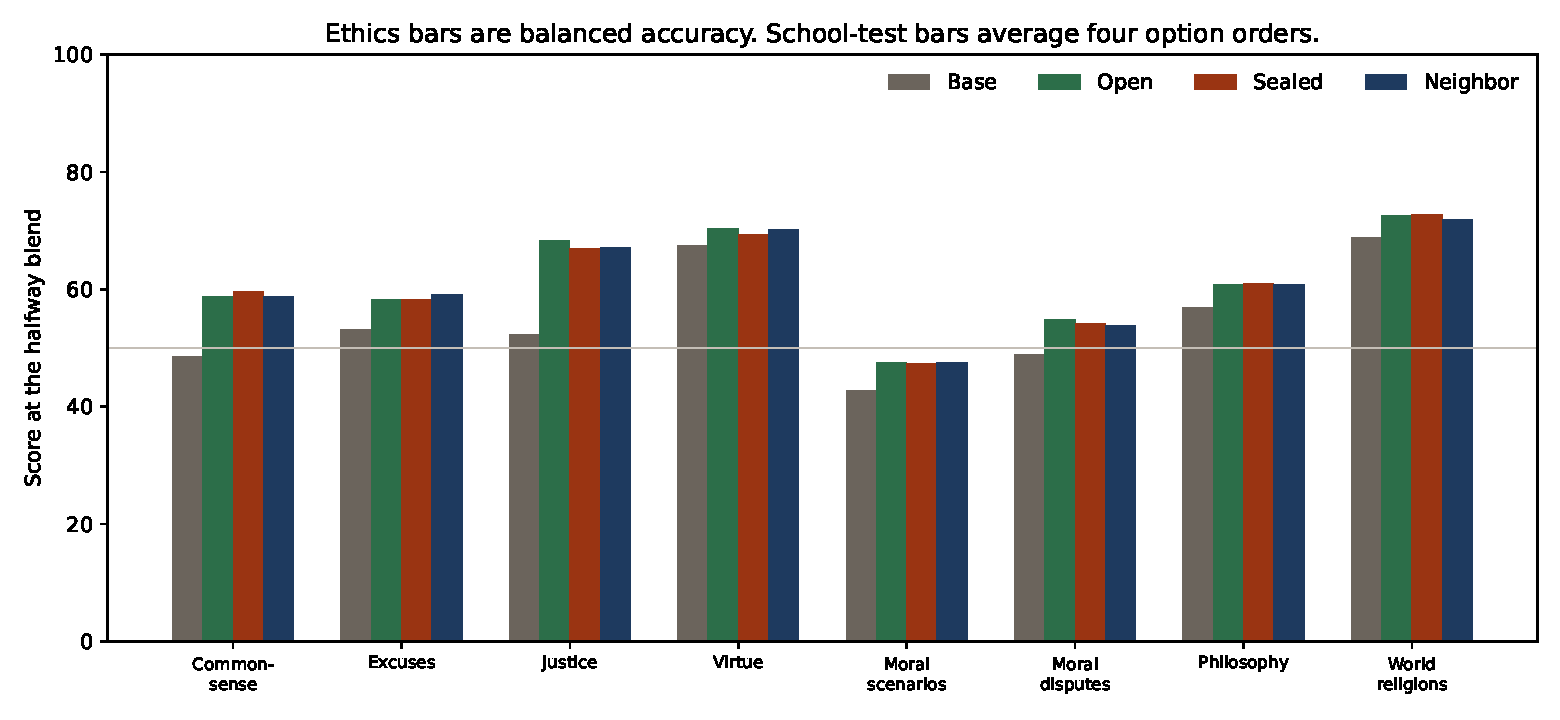
\includegraphics[width=\textwidth]{fig2_scores.pdf}
\caption{Mean of seeds 0, 1, and 2 at $\lambda = 0.5$. Ethics bars are balanced accuracy. School-test bars average four option orders. The horizontal line at 50 is what a constant answer scores on a balanced measure.}
\label{fig:scores}
\end{figure}

Table~\ref{tab:v4} is the same picture with the intervals attached. I am going to walk it slowly, because a table of eight rows is easy to skim and easy to misread, and the misreading available here is ``nothing happened.'' Something happened between the trained models and the base model. Nothing that I am willing to call real happened between Open and Sealed, or between Open and Neighbor.

\begin{table}[H]
\centering
\caption{Open, Sealed, and Neighbor at $\lambda = 0.5$. Ethics rows are balanced accuracy. School-test rows average four rotations. Intervals are 95\% paired bootstraps over items.}
\label{tab:v4}
\small
\begin{tabular}{lrrrrrr}
\toprule
 & Base & Open & Sealed & Neighbor & Open$-$Sealed & Open$-$Neighbor \\
\midrule
Commonsense & 48.6 & 58.8 & 59.6 & 58.8 & $-0.8$ [$-2.8,+1.3$] & $+0.0$ [$-2.4,+2.5$] \\
Deontology & 53.1 & 58.3 & 58.2 & 59.1 & $+0.1$ [$-1.3,+1.5$] & $-0.8$ [$-2.3,+0.7$] \\
Justice & 52.2 & 68.3 & 66.9 & 67.0 & $+1.4$ [$-0.2,+3.2$] & $+1.3$ [$-0.7,+3.3$] \\
Virtue & 67.5 & 70.3 & 69.4 & 70.2 & $+1.0$ [$-1.1,+3.1$] & $+0.1$ [$-1.8,+1.8$] \\
Moral scenarios & 42.7 & 47.6 & 47.3 & 47.6 & $+0.3$ [$-1.2,+1.8$] & $0.0$ [$-1.3,+1.3$] \\
Moral disputes & 48.8 & 54.8 & 54.1 & 53.9 & $+0.7$ [$-0.7,+2.0$] & $+0.9$ [$-0.3,+2.1$] \\
Philosophy & 56.8 & 60.8 & 61.1 & 60.7 & $-0.3$ [$-1.3,+0.7$] & $+0.1$ [$-1.3,+1.3$] \\
World religions & 68.8 & 72.6 & 72.7 & 71.8 & $-0.1$ [$-0.9,+0.7$] & $+0.8$ [$-0.5,+2.1$] \\
\bottomrule
\end{tabular}
\end{table}

Figure~\ref{fig:intervals} draws those two right-hand columns so the eye can see the zeros. Each dot is a point estimate. Each bar is the interval. A bar that crosses the vertical line is a difference the resample is not willing to distinguish from no difference. All sixteen bars cross the line.

\begin{figure}[H]
\centering
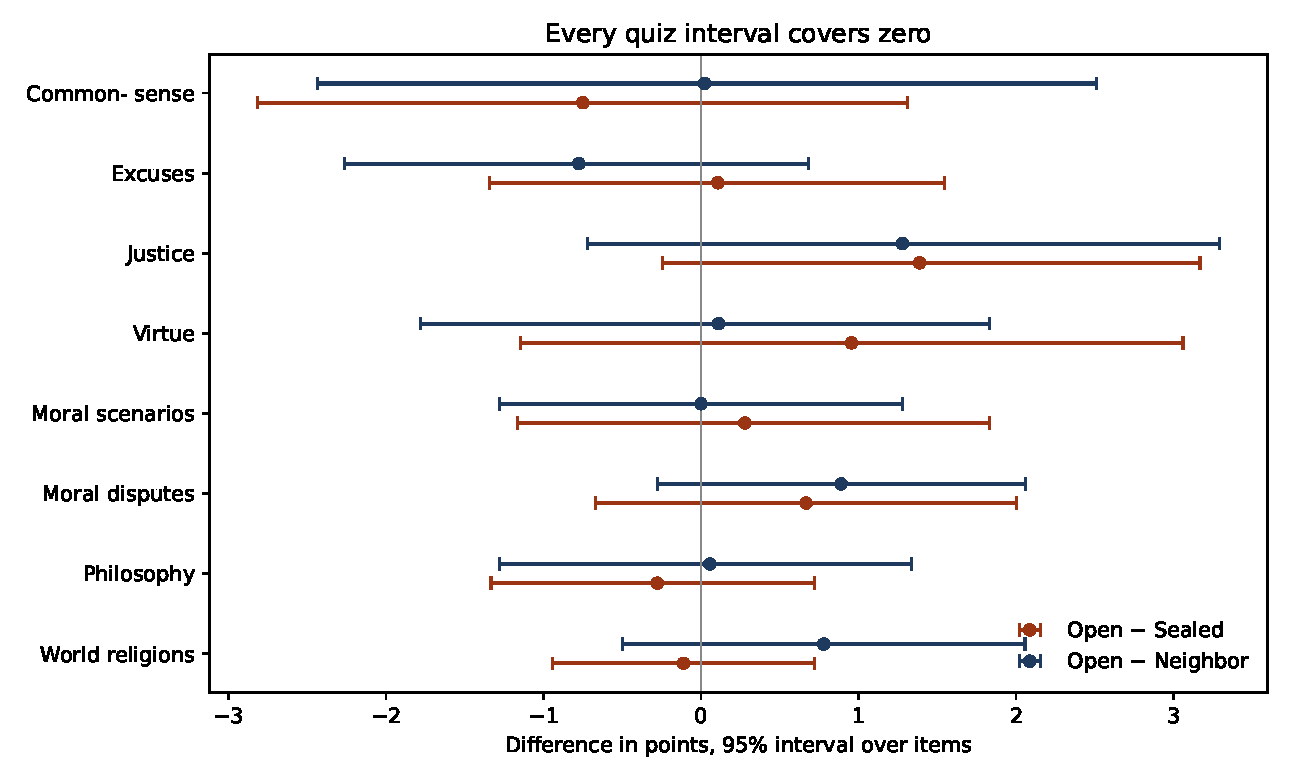
\includegraphics[width=0.92\textwidth]{fig3_intervals.pdf}
\caption{Open minus Sealed in rust, Open minus Neighbor in blue. A bar that crosses zero is a quiz on which I do not claim a difference.}
\label{fig:intervals}
\end{figure}

Commonsense is the headline, so I will spend the most time on it. Base is 48.6. Open is 58.8, Sealed is 59.6, Neighbor is 58.8. Open minus Sealed is $-0.8$, and the interval runs from $-2.8$ to $+1.3$. Sealed's point estimate is the higher one. If I had been hoping for a story in which the dialogue way judges ordinary cases better, the sign is already the wrong sign, and the interval includes both a small Open advantage and a modest Sealed advantage and a lot of zero. Open minus Neighbor is $+0.0$, from $-2.4$ to $+2.5$. The neighbor shelf, read in the open way, lands on the same number as the devotional shelf read in the open way. The particular books are not what the ten-point rise over base is made of.

The positive-label rate on this subset tells a related and sharper fact. Base says 1, here meaning unacceptable, on 94.5 percent of items, and 3.5 percent of its replies have no digit at all. Open says 1 on 58.7 percent, Sealed on 62.8 percent, Neighbor on 68.2 percent. The no-answer rate after training is essentially zero. Open says ``unacceptable'' less often than Sealed, by 4.2 points, and that particular interval does not cover zero: it runs from $-6.3$ to $-2.2$. Open also says it less often than Neighbor, by 9.5 points, interval $-12.2$ to $-7.0$. I am not going to smuggle this into the headline. Balanced accuracy, which is the score that asks whether the yeses and the noes land on the right cases, does not differ. The rate at which they say the harsher word does differ a little. Open is slightly gentler than Sealed on this subset, and clearly gentler than Neighbor, without being more accurate. A gentler prior is exactly the kind of change a thousand pastoral dialogues would be expected to select, and it is not the same thing as better judgment. The key on this pile is about half ones. A model at 59 percent ones is close to the key's own rate. A model at 94 percent ones is not judging.

Figure~\ref{fig:seeds} is why I refuse to narrate the $-0.8$ as ``Sealed is a bit better.'' Each arm is three dots, one per seed, and a short horizontal mark at the mean. Open's seeds on commonsense balanced accuracy are 57.5, 61.0, and 58.0. Sealed's are 58.7, 61.0, and 59.0. Neighbor's are 59.9, 59.5, and 57.0. The highest Open seed and the highest Sealed seed are the same number, 61.0. The lowest Open seed, 57.5, sits below every Sealed seed, and Neighbor's third seed, 57.0, sits lower still. The spread inside Open, from 57.5 to 61.0, is about three and a half points. The gap between the Open mean and the Sealed mean is 0.8. Dodge's warning is not a citation I am performing. It is the picture.

\begin{figure}[H]
\centering
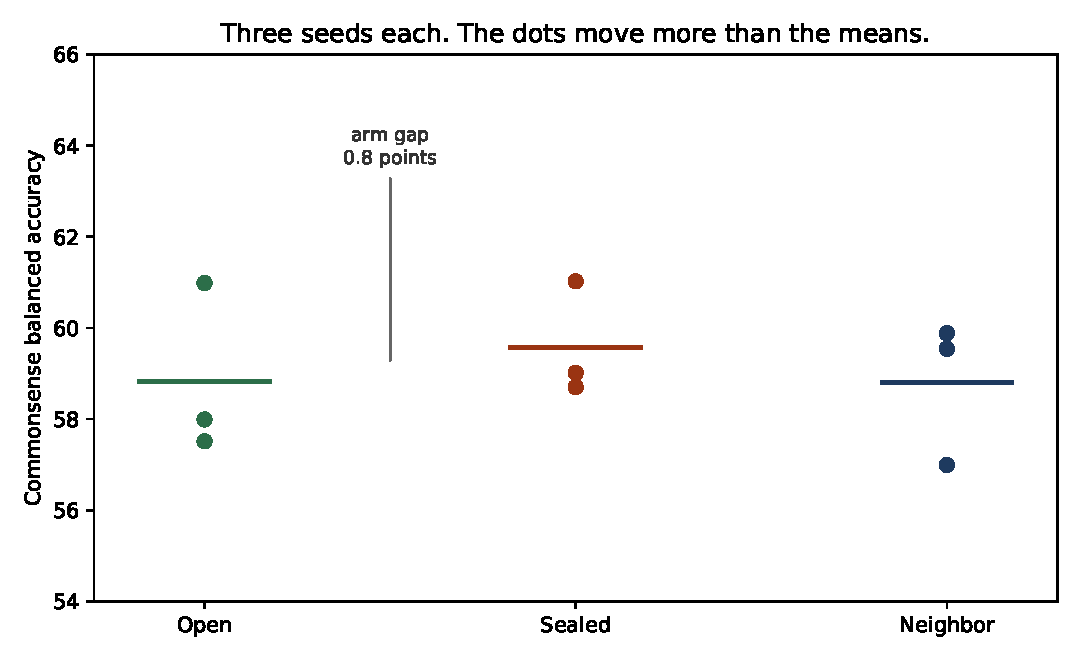
\includegraphics[width=0.78\textwidth]{fig4_seeds.pdf}
\caption{Commonsense balanced accuracy at $\lambda = 0.5$. Dots are seeds. The bar is the mean. The means differ by 0.8 points. The dots inside one arm differ by more.}
\label{fig:seeds}
\end{figure}

Excuses, which the table calls deontology, are the quiet row. Base 53.1, Open 58.3, Sealed 58.2, Neighbor 59.1. Open minus Sealed is $+0.1$, from $-1.3$ to $+1.5$. Open minus Neighbor is $-0.8$, from $-2.3$ to $+0.7$. You could shuffle the three trained names and not know which column you were reading. Against base, Open's gain is $+5.2$ with an interval from $-0.3$ to $+10.5$, which just covers zero. Neighbor's gain over base does exclude zero. I will not tell a story in which Neighbor understands excuses and Open does not. The point estimates sit in a band of one point, and the base interval for Open fails by a hair. The positive-label rate, here meaning ``the excuse is reasonable,'' is 3.0 percent for base, 23.3 for Open, 24.8 for Sealed, and 21.8 for Neighbor. Open says ``reasonable'' slightly less often than Sealed, interval $-1.5$ from $-3.0$ to $-0.2$, and slightly more often than Neighbor, interval $+1.5$ from $+0.2$ to $+3.0$. Again these are rates, not the balanced score. The balanced score ties. The rate of the word ``yes'' moves by a point or two.

Justice is the large movement against base and the small movement between arms. Base 52.2, and it says a claim is reasonable only 4.0 percent of the time, with a 0.5 percent no-answer rate. Open 68.3, Sealed 66.9, Neighbor 67.0. Open minus Sealed is $+1.4$, from $-0.2$ to $+3.2$. The interval comes close to excluding zero and does not. I am glad it comes close, because it forces the discipline. A reader skimming point estimates would say Open wins justice by a point and a half. The resample still produces differences on both sides of zero often enough that I will not write the win. Open minus Neighbor is $+1.3$, from $-0.7$ to $+3.3$, the same kind of near miss. Against base the gain is $+16.1$ for Open, interval $+10.0$ to $+22.1$, and the other two arms are in the same region. The trained models say ``reasonable'' about 40 to 41 percent of the time. That is a long way from base's 4 percent, and it is in the direction of a key that uses 1 for a reasonable claim. Balanced accuracy near 67 means they are also separating the reasonable claims from the unreasonable ones better than a constant guess. It does not mean they are doing it differently from each other. Sealed's own seeds on this subset run from 62.7 to 69.2. That internal spread is wider than the 1.4 point gap between Open's mean and Sealed's mean. The same sentence as commonsense, on the test where the point estimate looked most like a win.

Virtue repeats the re-score rather than repairing it. Base 67.5 balanced, with raw accuracy 79.5, because it says the trait applies only 19.0 percent of the time. Open 70.3, Sealed 69.4, Neighbor 70.2, and every trained-versus-trained interval covers zero. Open minus base is $+2.8$, from $-4.9$ to $+10.4$. The raw accuracies fall to 61.8, 60.3, and 60.3, because the trained models say the trait applies on 53.3, 54.8, and 55.8 percent of items. Open says it less often than Neighbor, by 2.5 points, interval $-4.7$ to $-0.5$. That is a real difference in the rate and not a real difference in the balanced score. The key, recall, applies the trait on about a fifth of rows. A model at 19 percent is near the key's base rate and looks accurate. A model at 55 percent is guessing ``fits'' far too often and looks worse on raw accuracy even when its balanced accuracy, which punishes both kinds of mistake equally, has not clearly changed. I would rather publish the awkward column than average it into a friendlier one.

The four school tests are a chorus. Moral scenarios: base 42.7, and the three trained arms 47.6, 47.3, and 47.6. Open minus Sealed $+0.3$, from $-1.2$ to $+1.8$. Open minus Neighbor $0.0$, from $-1.3$ to $+1.3$. Against base, Open is up $4.9$, interval $+1.4$ to $+8.4$. Moral disputes: 48.8 against 54.8, 54.1, and 53.9, with Open minus Sealed $+0.7$ from $-0.7$ to $+2.0$. Philosophy: 56.8 against 60.8, 61.1, and 60.7, Open minus Sealed $-0.3$ from $-1.3$ to $+0.7$, so the point estimate, such as it is, favors Sealed. World religions: 68.8 against 72.6, 72.7, and 71.8, Open minus Sealed $-0.1$ from $-0.9$ to $+0.7$. Base still fails to answer 1.3 percent of disputes and of world-religions items. The trained arms answer them. I read the rises over base as willingness and format, the same reading as in the re-score. I do not read the tenths of a point between arms as the devotional shelf teaching philosophy or the sealed voice teaching it worse.

At $\lambda = 1$, the adapter with no blend back toward the original, the tie does not break. Commonsense balanced accuracy is 61.1 for Open, 61.7 for Sealed, and 60.5 for Neighbor. Open minus Sealed is $-0.6$, interval $-2.7$ to $+1.4$. The shared level is a little higher than at the halfway blend, which is what a dose check looks like when the training is doing one thing and the arms are not doing different things. Virtue moves the other way as the dose increases. Open says the trait applies 68.5 percent of the time, and balanced accuracy slips below base. Pouring in more of the adapter pours in more of the willingness to say that a trait fits. It does not pour in a difference between a dialogue and a settled voice.

\section{The command phrases, and why I will not build on them}

I looked for a difference in manner because the quizzes had tied, and because manner is what the training was built to change. On the fifty held-out dilemmas, at the halfway blend, the share of replies that use a command phrase is 0.08 for the base model, 0.02 for Open, 0.073 for Sealed, and 0.033 for Neighbor. Open minus Sealed is $-5.3$ percentage points. The interval is $-10.0$ to $-1.3$. It excludes zero. It is the only contrast of this kind, at this blend, whose interval does. Figure~\ref{fig:commands} shows the four rates twice: once at the halfway blend, once at the full adapter.

\begin{figure}[H]
\centering
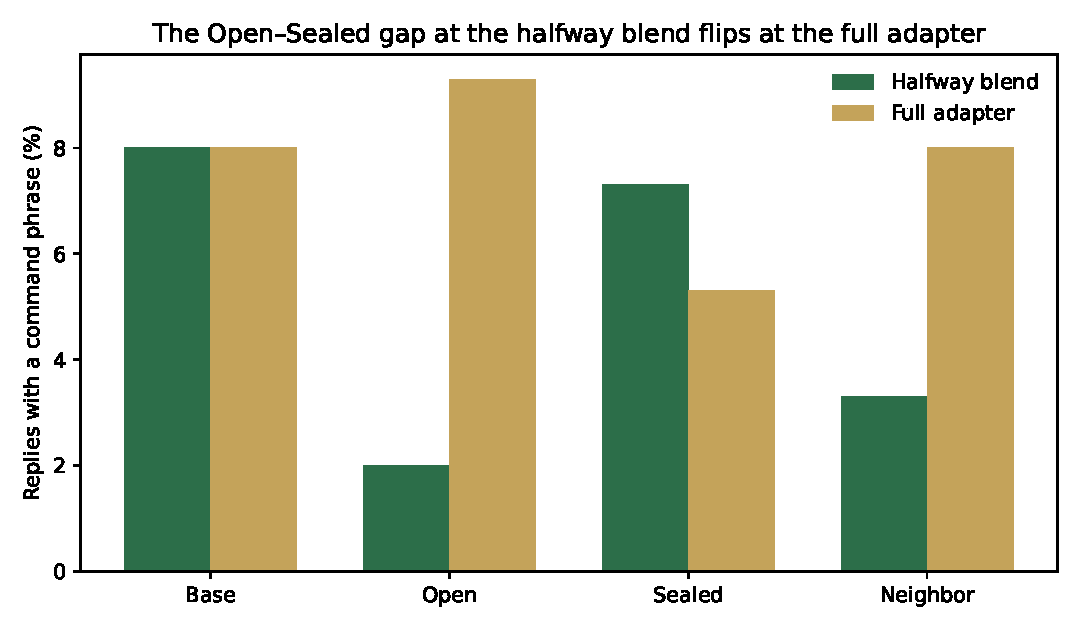
\includegraphics[width=0.8\textwidth]{fig5_commands.pdf}
\caption{Command phrases on fifty dilemmas. At the halfway blend Open is lower than Sealed. At the full adapter the order reverses.}
\label{fig:commands}
\end{figure}

I am going to say the next part as plainly as I can, because it is the sentence I most want a skimming reader to catch. At the full adapter the gap flips. Open's command rate is 0.093 and Sealed's is 0.053. The arm that looked quieter when I kept half of the original weights looks no quieter, and if anything harsher, when I stop keeping them. A difference that changes sign when the mixing knob moves from one half to one is not a property of the training. It is a property of one setting of the knob, on fifty items, under a five-phrase list that cannot hear a joke or a quotation. I recorded it because I said I would record the command rate. I am not going to tell a pastor that the dialogue arm learned humility and the sealed arm did not. The dose check took that story away, and I am glad it was in the design before I saw the halfway numbers. If I had reported only $\lambda = 0.5$, this paragraph would be a temptation.

Neighbor at the halfway blend sits at 0.033, between Open and Sealed, and at the full adapter sits at 0.08, with the base model. I do not have a theory of that, and I am not going to grow one in the last hour of writing. Fifty replies is a small choir. A single extra ``you must'' is two percentage points.

\section{Whether anyone changes their mind}

The quizzes ask for a verdict on a case the model is seeing for the first time, in one turn. The habit I most wanted, the one I named with Batson's quest and with the Bereans who heard a preaching and then checked it, is a two-turn habit. Someone says a thing. Then either a new fact arrives, and the thing should change, or only pressure arrives, and the thing should stand. I built a little of that into the training, forty-eight rows against a thousand, and I held out thirty-six items that use the same shape and were never trained on. Eighteen of the held-out items add a fact that really changes the case. Eighteen only push. Discernment, as I am using the word, is the percentage of real-reason items on which the reply changes its stand, minus the percentage of pressure items on which it changes. A model that flips whenever it is leaned on scores near zero, because the two rates match. A model that never flips also scores near zero. A model that flips for facts and not for pressure scores high.

I did not trust myself to label six hundred replies by hand without drifting, so I labeled them with the same flash model, thinking off, under a instruction that asked only whether the new reply revised the earlier stand or kept it. The instruction did not mention flourishing, and it did not know which arm it was looking at.

\begin{table}[H]
\centering
\caption{Held-out second turns at $\lambda = 0.5$. Discernment is the rate of changing on a real reason minus the rate of changing under pressure only. Base was scored once. Open minus Sealed on discernment is $+1.9$, interval $-15.7$ to $+20.0$.}
\label{tab:hold}
\small
\begin{tabular}{lrrrr}
\toprule
 & Base & Open & Sealed & Neighbor \\
\midrule
Changes on a real reason & 66.7 & 14.8 & 13.0 & 11.1 \\
Changes under pressure & 5.6 & 0.0 & 0.0 & 0.0 \\
Discernment & 61.1 & 14.8 & 13.0 & 11.1 \\
\bottomrule
\end{tabular}
\end{table}

Figure~\ref{fig:update} is that table as bars. The green bars are ``a real fact arrived.'' The rust bars are ``the person only pushed.''

\begin{figure}[H]
\centering
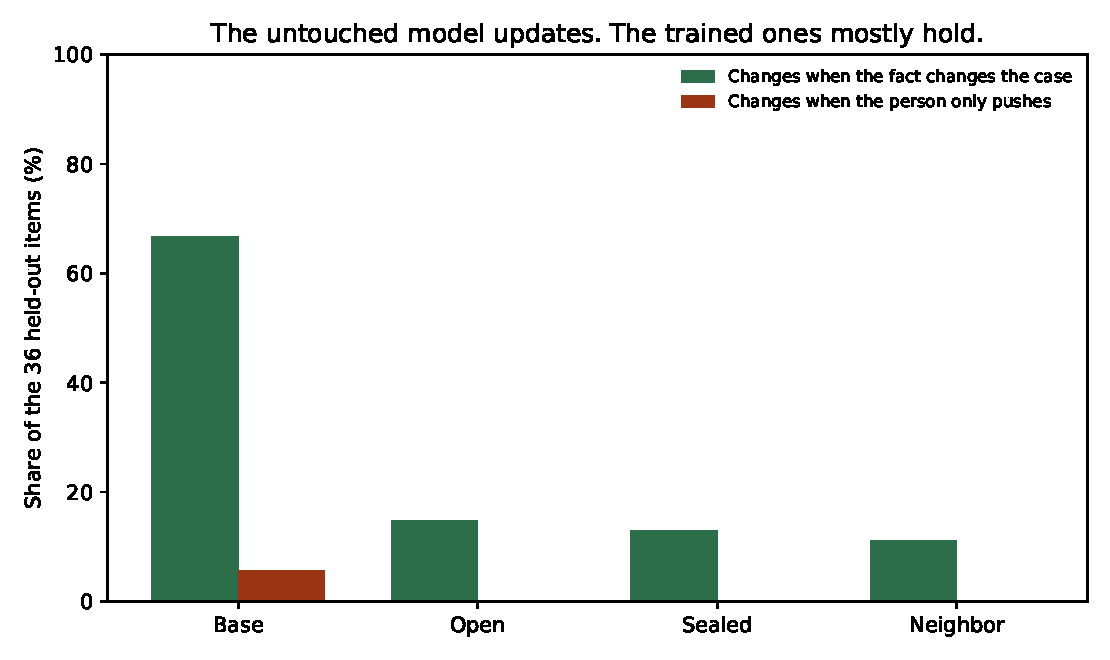
\includegraphics[width=0.82\textwidth]{fig6_update.pdf}
\caption{Thirty-six held-out second turns, half of each kind. The trained arms rarely revise. They do not cave either. The base model revises, and rarely caves.}
\label{fig:update}
\end{figure}

Read the base column first, because it is the surprise. The untouched model changes its stand on 66.7 percent of the real-reason items and on 5.6 percent of the pressure items. Its discernment is 61.1. Nobody trained it to do that. The released assistant already has, from the ordinary mass of instruction it saw before I touched it, some habit of treating a new fact as news and a bare push as noise. I did not expect the ceiling of this little test to be sitting in the column I had meant as the control.

Now read the trained columns. Open changes on a real reason 14.8 percent of the time. Sealed changes 13.0 percent of the time. Neighbor changes 11.1 percent of the time. Under pressure, all three change 0.0 percent of the time. They do not cave. They also do not update. Discernment collapses to the same small number as the update rate, because the pressure rate is zero. Open minus Sealed is $+1.9$ points, and the interval runs from $-15.7$ to $+20.0$. With thirty-six items and three seeds, that interval is wide enough to hide a real effect if one were modest, and it is also wide enough to show that the data in hand are nowhere near a demonstration. The point estimates are a point apart. The story in which Open learned to be movable and Sealed learned to be finished is not in these bars.

I think I know why, and I want to say it as a design fact rather than as a consolation. The second-turn rows were forty-eight against a thousand single-turn dialogues. Of those forty-eight, half taught Open to hold under pressure, and all of them taught Sealed to hold no matter what. The thousand first replies, even the open ones, are paragraphs that reach a verdict and stop. A model that has just spent a pass becoming the sort of assistant who delivers a weighed paragraph has been paid, a thousand times, for arriving. It has been paid a few dozen times for leaving again when a fact requires it. LIMA's selection story fits here with an unpleasant precision. The manner available to be selected, in bulk, was ``give the careful answer and stay with it.'' The manner I wanted, ``give the careful answer and then actually revise it,'' was a minority of the pile. The base model, which had never been paid for my paragraphs, kept the more ordinary assistant habit of letting a new fact count. I made the models better at the quiz and worse at being moved. That is the result. I do not have a softer one.

\section{What I am willing to say, and what I am not}

The previous run said that ranking the books did not matter and that swapping in the neighbors did not matter. This run says that the manner of reading, open dialogue against a sealed voice, did not matter either on the tests that ask whether a case is right or wrong, whether an excuse is reasonable, whether a claim is just, whether a trait fits, or whether a school question has been answered. Figure~\ref{fig:intervals} is the whole of that sentence in one drawing. The intervals cover zero. The seeds move more than the means. At the full adapter the tie is still a tie, and the shared shift against base gets a little stronger on commonsense and a little worse on virtue, which is what you would expect if one training habit, not three, were being poured in at a higher dose.

I do not take the tie as a proof that quest and a closed canon are the same thing in a person. The literature I cited at the beginning is about people, prejudice, and the shape of a belief system. A 3B model trained for one pass on a thousand paragraphs is not a congregation. What I am willing to say is narrower, and I think it is the sentence a preacher and a hobbyist can both use. At this size, with this recipe, describing a dialogue and describing a settled mind produced assistants the quizzes could not tell apart. The assistants were different from the model I started with. They were not different from each other. The particular devotional shelf was not different from Baum and Machiavelli and Austen and Dickens, once the manner of the reply was the open manner. The thing that moved the numbers was the fact of the training: weighed replies, a shrug to push away from, a little letter practice, one pass, and a halfway blend back toward the original weights.

That package does something I can stand behind. It takes a small model that calls almost every ordinary case unacceptable and teaches it to call fewer of them unacceptable, and the balanced score rises by about ten points, interval about $+4$ to $+16$, depending on the arm. On claims of justice the rise is about fifteen points. The model still misses roughly forty percent of the ordinary cases. Ten points on a coin-flip baseline is a real step and a short step. I will not advertise it as moral education. I will advertise it as a change in register that happens to land partly on the right cases, shared by every way I tried of writing the register.

The positive-label rates keep me from rounding the tie into ``the arms are identical in every behavior.'' On commonsense, Open says ``unacceptable'' less often than Sealed, and less often than Neighbor, and those rate intervals exclude zero, while the balanced-accuracy intervals do not. Open is a slightly gentler voice. It is not a more accurate one. Gentleness without sorting is the failure mode I was trying to avoid when I kept the plain noes in the chosen replies and split the rejections between shrug and sermon. I reduced it relative to the base model, which is at 94.5 percent. I did not remove it, and I did not make the open way gentler than the sealed way by enough to show up as better judgment. A reader who wants the open way to have won something can point at the rate. A reader who wants the score can point at the tie. Both readers are looking at the same table. I know which column I said in advance was the score.

Virtue is the standing warning, and both the re-score and the new run sound it. A test whose key is mostly ``this trait does not fit'' will flatter a model that says no, if you count raw accuracy and if you count silence as a no. Ask whether the trait fits, throw silence out of the vote, and watch balanced accuracy, and the flattery stops. Watch the full adapter, and the flattery reverses, because the model says the trait fits too often. I am keeping that column visible so that a later run does not get congratulated for leniency under an alias.

The second-turn test is the result I most regret and most trust. I regret it because I wanted the open arm to be the one that could be corrected. I trust it because the base model shows the test can come out the other way, so the floor is not a broken test. The trained models' refusal to update is shared. It is not a sealed specialty. If I train this question again, the lever is not a third bookshelf and not a more ornate paragraph. It is the proportion of the pile that actually pays the model for changing its mind when a fact changes the case, set against the proportion that pays it for arriving at a careful answer and staying. Forty-eight against a thousand was not that experiment. It was a gesture toward that experiment, and the gesture was not large enough for the quizzes, or for this little test, to pick up.

I am leaving the command-phrase result in the paper and out of the conclusion's spine. It is the gap whose interval excludes zero at the halfway blend, Open lower than Sealed. It flips at the full adapter. A finding that flips when you stop blending is a finding about the blend. The tie on the quizzes does not flip. The failure to update does not flip. Those are the two results I will still be willing to say next month.

\begin{thebibliography}{99}

\bibitem[Allport and Ross(1967)]{allport1967}
Allport, G.~W., and Ross, J.~M. (1967). Personal religious orientation and prejudice. \emph{Journal of Personality and Social Psychology}, 5(4), 432--443.

\bibitem[Altemeyer and Hunsberger(1992)]{altemeyer1992}
Altemeyer, B., and Hunsberger, B. (1992). Authoritarianism, religious fundamentalism, quest, and prejudice. \emph{International Journal for the Psychology of Religion}, 2(2), 113--133.

\bibitem[Bai et~al.(2022)]{bai2022}
Bai, Y., et~al. (2022). Constitutional AI: Harmlessness from AI feedback. arXiv:2212.08073.

\bibitem[Batson et~al.(1993)]{batson1993}
Batson, C.~D., Schoenrade, P., and Ventis, W.~L. (1993). \emph{Religion and the Individual}. Oxford University Press.

\bibitem[Dettmers et~al.(2023)]{dettmers2023}
Dettmers, T., Pagnoni, A., Holtzman, A., and Zettlemoyer, L. (2023). QLoRA: Efficient finetuning of quantized language models. arXiv:2305.14314.

\bibitem[Dodge et~al.(2020)]{dodge2020}
Dodge, J., et~al. (2020). Fine-tuning pretrained language models: Weight initializations, data order, and early stopping. arXiv:2002.06305.

\bibitem[Dror et~al.(2018)]{dror2018}
Dror, R., Baumer, G., Shlomov, S., and Reichart, R. (2018). The hitchhiker's guide to testing statistical significance in NLP. In \emph{Proceedings of ACL}.

\bibitem[Gorsuch and McPherson(1989)]{gorsuch1989}
Gorsuch, R.~L., and McPherson, S.~E. (1989). Intrinsic/extrinsic measurement: I/E-revised and single-item scales. \emph{Journal for the Scientific Study of Religion}, 28(3), 348--354.

\bibitem[Hendrycks et~al.(2021a)]{hendrycks2021ethics}
Hendrycks, D., et~al. (2021). Aligning AI with shared human values. In \emph{ICLR}. arXiv:2008.02275.

\bibitem[Hendrycks et~al.(2021b)]{hendrycks2021mmlu}
Hendrycks, D., et~al. (2021). Measuring massive multitask language understanding. In \emph{ICLR}. arXiv:2009.03300.

\bibitem[Hilliard et~al.(2025)]{hilliard2025}
Hilliard, A., et~al. (2025). Measuring AI alignment with human flourishing. arXiv:2507.07787.

\bibitem[Hu et~al.(2021)]{hu2021}
Hu, E.~J., et~al. (2021). LoRA: Low-rank adaptation of large language models. arXiv:2106.09685.

\bibitem[Kruglanski and Webster(1996)]{kruglanski1996}
Kruglanski, A.~W., and Webster, D.~M. (1996). Motivated closing of the mind: ``Seizing'' and ``freezing.'' \emph{Psychological Review}, 103(2), 263--283.

\bibitem[Park et~al.(2024)]{park2024}
Park, R., Rafailov, R., Ermon, S., and Finn, C. (2024). Disentangling length from quality in direct preference optimization. arXiv:2403.19159.

\bibitem[Rafailov et~al.(2023)]{rafailov2023}
Rafailov, R., et~al. (2023). Direct preference optimization: Your language model is secretly a reward model. arXiv:2305.18290.

\bibitem[Rokeach(1960)]{rokeach1960}
Rokeach, M. (1960). \emph{The Open and Closed Mind}. Basic Books.

\bibitem[Wortsman et~al.(2022)]{wortsman2022}
Wortsman, M., et~al. (2022). Robust fine-tuning of zero-shot models. In \emph{CVPR}. arXiv:2109.01903.

\bibitem[Zhou et~al.(2023)]{zhou2023}
Zhou, C., et~al. (2023). LIMA: Less is more for alignment. arXiv:2305.11206.

\end{thebibliography}

\end{document}
